% ------------------------------------------------------------------
%  Main body (PRL format) -- no title/abstract/intro/conclusion yet.
%  Compile with paper/main.tex (revtex4-2).
% ------------------------------------------------------------------

\begin{figure}[t]
  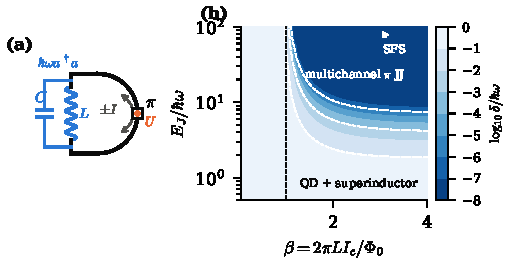
\includegraphics[width=\columnwidth]{../figs/fig_overview.pdf}
  \caption{\label{fig:overview}%
  (a) A superconducting loop closed by a $\pi$ junction (here an interacting dot
  with charging energy $U$) shares its inductance $L$ with an LC mode; the two
  degenerate states carry opposite persistent currents $\pm I$.
  (b) Tunnel splitting $\delta$ between the two current-carrying states in the
  plane of the screening parameter $\beta$ and the quantum parameter $E_J/\hbar\omega$
  [Eq.~\eqref{eq:BO} with the DMRG $E(\varphi)$ of the $U=2t$ junction]. White
  lines: $\delta/\hbar\omega=10^{-6},10^{-3},10^{-1}$; dashed: classical threshold $\beta=1$.
  Labels: typical regimes of the platforms discussed in the text.}
\end{figure}

\paragraph*{Model.}
We consider a superconducting (SC) loop interrupted by a single Josephson
element and threaded by the magnetic flux of one lumped LC mode
[Fig.~\ref{fig:overview}(a)],
\begin{equation}
  H = \hbar\omega\, a^\dagger a + H_{\rm ring}\!\left[\varphi_{\rm cl} + g\,(a+a^\dagger)\right].
  \label{eq:H}
\end{equation}
$H_{\rm ring}[\varphi]$ is a microscopic lattice Hamiltonian of the loop:
an $s$-wave BCS chain $-t\sum_{r\sigma}(c^\dagger_{r+1\sigma}c_{r\sigma}+{\rm h.c.})
+\Delta\sum_r(c^\dagger_{r\uparrow}c^\dagger_{r\downarrow}+{\rm h.c.})$
closed by a junction, which is either a weak bond $t_J$ or an Anderson
impurity (level $\epsilon_d$, Hubbard repulsion $U$) tunnel-coupled to both banks.
The total Peierls phase on the loop is placed on one junction bond,
$-t_J\sum_\sigma e^{i\varphi}c^\dagger_{1\sigma}c_{0\sigma}+{\rm h.c.}$.
An electron phase $\varphi=\pi$ corresponds to one superconducting flux quantum
$\Phi_0=h/2e$. The vector potential of the mode enters through the gauge-invariant
displacement operator $D=e^{ig(a+a^\dagger)}$, so diamagnetic ($A^2$) terms are
included to all orders. $g=2\pi\Phi_{\rm zpf}/\Phi_0^{(e)}$ is the electron phase
generated by the zero-point flux of the mode, and $\varphi_{\rm cl}$ is a static
external flux. For a lumped resonator of impedance $Z$, galvanically sharing
its inductance with the loop, $(2g)^2=\pi Z/R_Q$ with $R_Q=h/4e^2$.

The only property of $H_{\rm ring}$ that enters below is its ground-state
energy at fixed phase,
\begin{equation}
  E(\varphi)=\sum_{m\ge 0}E_m\cos m\varphi .
  \label{eq:harm}
\end{equation}
Even harmonics ($m=2,4,\dots$) describe Cooper-pair tunnelling ($h/2e$
periodicity). The $m=1$ term is the single-electron ($h/e$) persistent
current of a mesoscopic ring~\cite{LossGoldbart1991} and is suppressed as $e^{-L/\xi}$. A
$0$-junction has $E_2<0$ and a $\pi$-junction has $E_2>0$. When a $0$-junction
is biased by $\Phi_0/2$, $\varphi_{\rm cl}=\pi/2$ maps $E_2\cos2\varphi\to-E_2\cos2\varphi$.
The two routes to a $\pi$ loop are therefore equivalent up to the odd harmonics,
which turn into an explicit symmetry-breaking term
$-E_1\sin\varphi$. In contrast, an intrinsic $\pi$-junction keeps
$E(\varphi)=E(-\varphi)$ exactly, since $H_{\rm ring}[0]$ is real
(time-reversal symmetry).

\paragraph*{Adiabatic reduction and Landau theory.}
For $\hbar\omega$ well below the Andreev gap $E_A$, the electrons follow the
flux adiabatically. To leading order in $\hbar\omega/E_A$, Eq.~\eqref{eq:H}
reduces to a single-particle problem for the dimensionless flux $X=a+a^\dagger$,
\begin{equation}
  H_{\rm BO}=\frac{\hbar\omega}{4}\left(P^2+X^2\right)+E(\varphi_{\rm cl}+gX),
  \qquad [X,P]=2i .
  \label{eq:BO}
\end{equation}
Equation~\eqref{eq:BO} is the Hamiltonian of an rf-SQUID~\cite{Friedman2000} whose inductive energy
is supplied by the mode. Writing it in the Cooper-pair phase
$\theta=2gX$ gives $4E_C n^2+\tfrac12E_L\theta^2+E(\theta/2)$ with
$E_L=\hbar\omega/8g^2$ and $E_C=\hbar\omega g^2$. A static field ($\langle a\rangle\neq0$),
i.e.\ a photon condensate carrying a persistent current
$I=-(2e/\hbar)\partial_\varphi E$, appears classically when the orbital response of the
ring at the symmetric point is paramagnetic and exceeds the stiffness of the mode,
\begin{equation}
  \beta\equiv\frac{2g^2\,|E''(\varphi_0)|}{\hbar\omega}>1,
  \qquad E''(\varphi_0)<0 .
  \label{eq:beta}
\end{equation}
For a pure $\pi$-junction, $\beta=8g^2E_J/\hbar\omega=2\pi L I_c/\Phi_0$, the
familiar screening parameter of the loop \cite{BKS1977,Tsuei2000}.
Equation~\eqref{eq:beta} is the single-loop form of the
photon-condensation criterion of Andolina \emph{et al.}~\cite{Andolina2020}: the no-go theorem
for a uniform cavity field~\cite{Andolina2019,Nataf2019} does not apply, because the mode couples to the
flux (curl of $\mathbf A$), and the instability requires a \emph{paramagnetic}
orbital response, which here comes from the $\pi$ shift.
Above threshold, the Landau free energy
$\mathcal F(X)=\hbar\omega X^2/4+E(gX)$ has two degenerate minima
$\pm X^\star$ carrying opposite currents $\pm I^\star$.

Two remarks fix the physical content of Eq.~\eqref{eq:beta}. First,
for a loop with its own geometric inductance $L_r$ and mutual inductance
$M\le\sqrt{L_rL_c}$ to the resonator, minimizing the static energy over the
resonator flux gives $\Phi_r^2/2L_r$: the static threshold is set by the
total loop inductance, and Eq.~\eqref{eq:H} is the $k=M/\sqrt{L_rL_c}\to1$
(galvanic) limit. Second, zero-point fluctuations of the mode do not
drive the transition; they oppose it. At finite $E_J/\hbar\omega$ the
ground state of Eq.~\eqref{eq:BO} is the symmetric superposition of the two
current-carrying states, split from its partner by a tunnelling gap
$\delta\sim\hbar\omega\,e^{-S}$ with an instanton action
$S\propto (E_J/\hbar\omega)\,s(\beta)$. A sharp quantum phase transition
with mean-field exponents is recovered in the scaling limit
$E_J/\hbar\omega\to\infty$ at fixed $\beta$, in which
$E_C/E_J=\beta(\hbar\omega)^2/(8E_J^2)\to0$. This is the analogue of the
classical-oscillator limit of the quantum Rabi model~\cite{Hwang2015}.

\paragraph*{Methods.}
We solve Eq.~\eqref{eq:H} without approximation by DMRG
(TeNPy~\cite{TeNPy}) on the full electron--photon Hilbert space. The ring is stored in folded
order next to a bosonic site (Fock cutoff $N_{\rm ph}$). Fermion parity and $S^z$
are conserved, and the electron--photon vertex is a three-site operator
$D\,c^\dagger_{1\sigma}c_{0\sigma}$. Benchmarks against exact BdG energies of the
non-interacting ring at $g=0$ agree to $10^{-14}$ at full bond dimension
($\chi=1024$). In production ($\chi=256$--$320$, $N_{\rm ph}=30$--$50$, discarded
Fock weight $<10^{-7}$) the ground-state energy error is $\lesssim3\times10^{-6}t$.
For a $4$-site ring with a photon, DMRG reproduces exact diagonalization and the identity
$\langle I\rangle=\hbar\omega\langle X\rangle/2g$ to $10^{-7}$. Excited states are obtained by DMRG
orthogonal to the ground state. We compare with (i) the self-consistent
electron$\times$photon product state (mean field, MF), and (ii) the adiabatic
Hamiltonian~\eqref{eq:BO}, with $E(\varphi)$ from BdG or from DMRG at fixed
$\varphi$, diagonalized exactly.

% RESULTS PARAGRAPHS ARE IN results.tex
\paragraph*{Breakdown of the product-state description.}
We first take the parameters of a Zeeman-polarized dot embedded in a short
BCS ring ($t=2$, $\Delta=0.6$, $L=11$, $\epsilon_{d\uparrow}=-0.3$,
$\epsilon_{d\downarrow}=3.7$, $t_J=0.5$, $\hbar\omega=0.02$). The
self-consistent product state predicts a current-carrying phase for
$g\gtrsim0.75$, with $\langle a^\dagger a\rangle\simeq1$--$1.4$ and
$|\langle I\rangle|\approx0.02$ [Fig.~\ref{fig:notebook}]. DMRG shows that this
phase is an artefact. The exact ground-state energy decreases monotonically with
$g$ and lies below the MF energy by up to $1.9\hbar\omega$ \TODO{update with
DMRG g=1.2}. The gap to the first excited state stays a sizeable fraction of
$\hbar\omega$ ($E_1-E_0=0.34\hbar\omega$ at $g=1.2$). The linear response to the
seed flux $\varphi_{\rm cl}=10^{-3}$ remains $\langle I\rangle\lesssim
4\times10^{-4}$, i.e.\ two orders of magnitude below the MF value. DMRG and
the adiabatic theory~\eqref{eq:BO} agree to within
$\lesssim2\%$ of $\hbar\omega$ in energy and to $<1\%$ in $E_1-E_0$.
The residual difference is the non-adiabatic (diagonal Born--Oppenheimer)
correction $\sim g^2\hbar\omega\,\hbar\omega/E_A$.

Two effects make the product state fail. (i) It is not gauge invariant~\cite{Li2020,Dmytruk2021}: with the full
Peierls phase on one bond, it renormalizes that bond by
$|\langle D\rangle|<1$ and so loses phase-\emph{independent} kinetic energy,
which the exact state recovers by following the flux adiabatically. (ii) Here
$E_J\simeq\hbar\omega$. The Landau free energy does develop a double well
for $g>0.58$, but its depth is below the zero-point energy, and the flux
distribution $P(X)$ stays essentially unimodal. A further subtlety
concerns ring size: since $L\lesssim\xi$, $E(\varphi)$ of this ring is dominated by the
single-electron harmonic, $E_1=2.1\times10^{-2}\gg E_2=2.0\times10^{-3}$
[Fig.~\ref{fig:junctions}(a)]. The instability would then be one of the normal
$h/e$ persistent current rather than of the Josephson junction. To isolate
Josephson physics we use rings with $L\gg\xi$ below
($t=1$, $\Delta=1$, $L=14$, giving $|E_1/E_2|\lesssim10^{-2}$).

\paragraph*{Half-flux-biased junction.}
For an ordinary weak link ($t_J=0.5$, $E_2=-0.056\,t$, Andreev gap
$0.77\,t$) biased by $\Phi_0/2$, Fig.~\ref{fig:halfflux} shows the full
DMRG solution at $E_J/\hbar\omega=10$ as a function of $\beta$.
\TODO{fill: DMRG current jumps to $|\langle I\rangle|\simeq I^\star$ at
$\beta\simeq1$, follows BO within ..., MF ...}
The flux distribution extracted from the photon reduced density matrix
evolves from a Gaussian centred at zero to a single displaced peak at
$\pm\Phi^\star$. The sign is fixed by the residual odd harmonic
$E_1=-5.4\times10^{-4}$, which tilts the double well by
$2|E_1|\sin\varphi^\star\approx10^{-3}t\approx0.2\hbar\omega$.
This tilt sets the splitting $E_1-E_0$ for $\beta>1.2$ in DMRG and BO alike. Without it,
$\delta/\hbar\omega$ would drop below $10^{-6}$ at $\beta=2$. The external-bias
route thus provides a current-carrying state whose direction is \emph{selected}
rather than spontaneously chosen. Its residual symmetry breaking is
$\propto e^{-L/\xi}$ for a homogeneous ring, but in practice it is limited
by the flux offset $\delta\Phi$.

\paragraph*{Interaction-driven $\pi$ junction without external flux.}
We now replace the weak link by an Anderson impurity at particle--hole
symmetry ($\epsilon_d=-U/2$, $t_J=0.5$) and set $\varphi_{\rm cl}=0$.
DMRG in the even and odd fermion-parity sectors
[Fig.~\ref{fig:junctions}(b,c)] gives the $0$--$\pi$ transition known for magnetic quantum dots~\cite{GlazmanMatveev1989,SpivakKivelson1991,Vecino2003,Karrasch2008,vanDam2006,Cleuziou2006,Delagrange2015}. For
$U<U_c\simeq0.9\,t$ the singlet (even) state is the ground state at $\varphi=0$
and the junction is a $0$-junction. For $U>U_c$ the Kramers doublet (odd sector)
is the ground state at all phases, and $E(\varphi)$ has its \emph{minimum} at the
Cooper-pair phase $\pi$. At $U=2t$ we find $E_2=+7.39\times10^{-3}t$, with
$|E_1|,|E_4|<10^{-4}t$: a pure $\pi$ junction, indistinguishable after
normalization from the half-flux-biased weak link [Fig.~\ref{fig:junctions}(a)].
The $\pi$ coupling decreases monotonically with $U$ ($E_2\propto U^{-1.3}$ for $4t\le U\le10t$), as expected for
cotunnelling through the singly occupied level.

Coupling this junction to the mode [Fig.~\ref{fig:udot}] gives the
transition without any static flux. Here $H_{\rm ring}$ is real and
$\langle I\rangle=0$ in every eigenstate, so the order is diagnosed by the
two lowest states. The splitting $\delta=E_1-E_0$ collapses and the
flux operator projected onto the quasi-degenerate doublet acquires the eigenvalues
$\pm\Phi^\star$. \TODO{fill DMRG numbers: at $E_J/\hbar\omega=10$, $\delta/\hbar\omega=$
... at $\beta=2$ and ... at $\beta=3$; $\Phi^\star$ ...}. In the photon-number basis
the DMRG ground state is a cat state: $P(\Phi)$ is bimodal with peaks at
$\pm\Phi^\star$, whose separation tracks the classical minimum. With
increasing $E_J/\hbar\omega$ the crossover sharpens into a pitchfork at
$\beta=1$ and $\delta$ vanishes exponentially [Fig.~\ref{fig:udot}(b)]. The
residual $\delta$ is the macroscopic tunnelling of a persistent current. Because
it is protected by time-reversal symmetry, it is the only
energy scale separating the two current directions. Each current state is
additionally Kramers degenerate in the spin of the dot. The low-energy manifold is
therefore a fourfold multiplet $\{\sigma=\uparrow,\downarrow\}\otimes\{\circlearrowright,\circlearrowleft\}$,
split only by $\delta$.

\paragraph*{Experimental scales.}
The two control parameters are
$\beta=2\pi L I_c/\Phi_0$ and $E_J/\hbar\omega$, related by
$\beta=2\pi(Z/R_Q)(E_J/\hbar\omega)$, with $E_J/h\simeq0.5\,{\rm GHz}\times I_c[{\rm nA}]$.
Three classes of $\pi$ elements span the phase diagram
[Fig.~\ref{fig:overview}(b)]:
(i) SFS junctions ($I_c\sim1$--$100\,\mu$A) reach $\beta>1$ with geometric
inductances of a few to a few hundred pH and $E_J/\hbar\omega\sim10^2$--$10^4$.
This is the classical limit, where the half-flux state is fully polarized,
consistent with the spontaneous currents observed in SFS
and $d$-wave $\pi$ loops~\cite{Tsuei2000,Ryazanov2001,Bauer2004}.
(ii) Quantum-dot $\pi$ junctions in the doublet regime
($I_c^\pi\sim0.1$--$10$\,nA) require $L\sim0.03$--$3\,\mu$H, i.e.\ superinductances
(Josephson-junction arrays, granular Al) as in fluxonium circuits~\cite{Manucharyan2009,Grunhaupt2019}; this is the $\pi$-qubit regime of Refs.~\cite{Ioffe1999,Yamashita2005,Feofanov2010}. These give
$E_J/\hbar\omega\sim1$: the ground state is the
cat state $(|{\circlearrowright}\rangle+|{\circlearrowleft}\rangle)/\sqrt2$ with
$\delta\sim0.1\hbar\omega$, and the transition appears as a dip in the
$|0\rangle\to|1\rangle$ frequency and a jump in the transition matrix element
$\langle0|\Phi|1\rangle$, accessible in two-tone spectroscopy.
(iii) Multichannel or gate-tunable $\pi$ junctions with
$I_c\sim50$--$200$\,nA in a high-kinetic-inductance loop ($L\sim2$--$10$\,nH,
$\omega/2\pi\sim2$--$5$\,GHz) give $\beta\sim1$--$3$ and $E_J/\hbar\omega\sim10$--$30$.
This is the regime of Figs.~\ref{fig:halfflux} and~\ref{fig:udot}: a well-defined
current-carrying state whose residual tunnelling $\delta/\hbar\omega\sim10^{-4}$--$10^{-8}$
remains a measurable macroscopic-quantum-tunnelling signature.
In the externally biased realization, the half-flux bias must be stable to
$|\delta\Phi|\ll\delta/2I^\star$, i.e.\ $\lesssim10^{-6}\Phi_0$ for the parameters above.
The interaction-driven realization has no such requirement.


% ------------------------------------------------------------------ figures
\begin{figure*}
  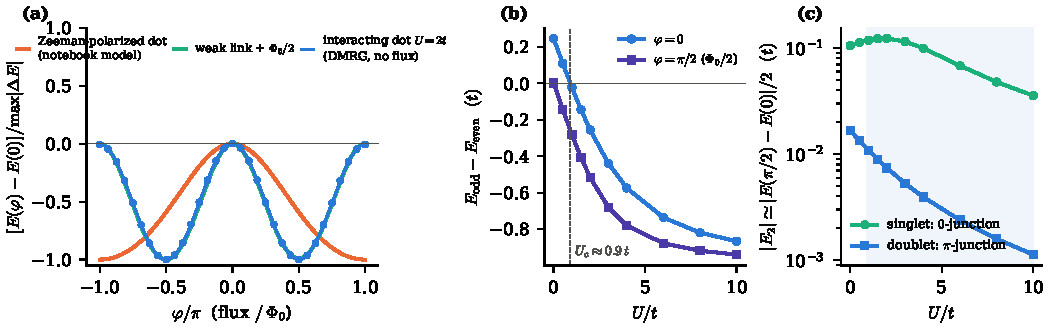
\includegraphics[width=\textwidth]{../figs/fig_junctions.pdf}
  \caption{\label{fig:junctions}%
  (a) Normalized ground-state energy of the loop versus the electron phase
  $\varphi$ (flux in units of $h/2e$) for three junctions:
  Zeeman-polarized dot in a short ring (dominated by the single-electron
  harmonic $\cos\varphi$), an ordinary weak link biased by $\Phi_0/2$, and an
  interacting dot at $U=2t$ without any bias (DMRG, symbols; line: cosine fit).
  (b) Parity competition $E_{\rm odd}-E_{\rm even}$ of the interacting-dot
  ring at $\varphi=0$ and $\varphi=\pi/2$ (DMRG, $L=14$, $\Delta=t$, $t_J=0.5t$).
  (c) Josephson energy $|E_2|$ in the singlet ($0$) and doublet ($\pi$)
  sectors. Shading: doublet ground state.}
\end{figure*}

\begin{figure}
  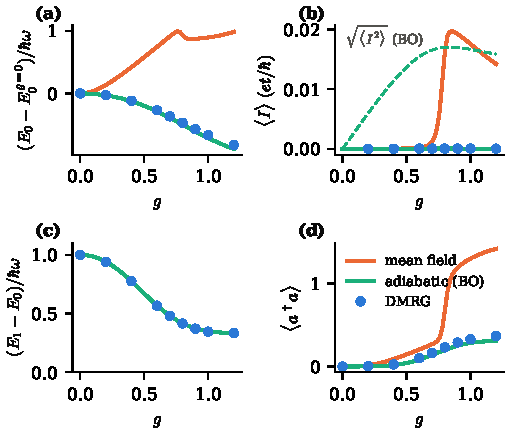
\includegraphics[width=\columnwidth]{../figs/fig_notebook_model.pdf}
  \caption{\label{fig:notebook}%
  Short ring with a Zeeman-polarized dot ($\hbar\omega=0.02$,
  $\varphi_{\rm cl}=10^{-3}$): mean field (MF, orange), adiabatic
  theory~\eqref{eq:BO} (green), and DMRG (symbols).
  (a) Ground-state energy, (b) current (dashed: rms current of the BO
  ground state), (c) gap to the first excited state, (d) photon number.}
\end{figure}

\begin{figure*}
  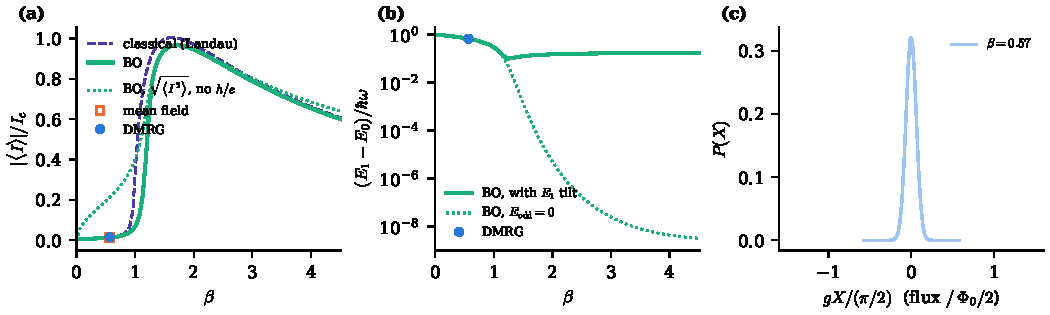
\includegraphics[width=\textwidth]{../figs/fig_weaklink_halfflux.pdf}
  \caption{\label{fig:halfflux}%
  Weak-link loop biased by $\Phi_0/2$, $E_J/\hbar\omega=10$.
  (a) Persistent current versus $\beta$: DMRG (circles), MF (squares), adiabatic
  theory with (solid) and without (dotted) the odd harmonics, classical
  Landau theory (dashed). (b) Splitting of the two lowest levels.
  (c) Flux distribution of the DMRG ground state, obtained from the photon reduced
  density matrix.}
\end{figure*}

\begin{figure*}
  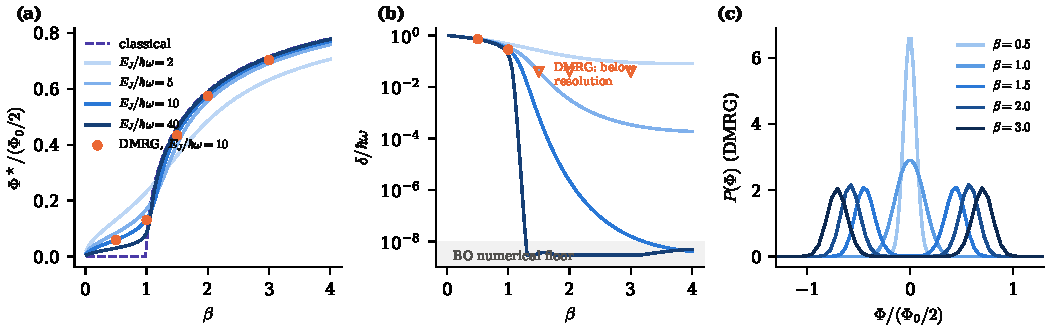
\includegraphics[width=\textwidth]{../figs/fig_udot_cavity.pdf}
  \caption{\label{fig:udot}%
  Interaction-driven $\pi$ loop ($U=2t$, no external flux).
  (a) Flux of the condensate $\Phi^\star$ (eigenvalue of the flux projected on the two
  lowest states) versus $\beta$ for increasing $E_J/\hbar\omega$ (lines: adiabatic
  theory with the DMRG $E(\varphi)$; circles: full DMRG at $E_J/\hbar\omega=10$;
  dashed: classical). (b) Tunnel splitting $\delta$ between the two
  current-carrying states. (c) Flux distribution of the DMRG ground state
  (a cat state for $\beta>1$).}
\end{figure*}

